\section{Entwurf eines vollständigen Konzepts} \label{sec:entwurfBIArchitektur}

\subsection{Auswahl der Komponenten} \label{sec:konzeption:evaAuswertung}
Mit den gewonnenen Erkenntnissen über die verschiedenen Azure Dienste, soll eine geeignete Auswahl für das Cloud-BI System getroffen werden. Eine zusammenfassende Einschätzung der Dienste in Bezug auf die Anforderungen kann in Tabelle~\ref{table:eva} gefunden werden. In den letzten drei Zeilen wird in Summen angeben, wie viele funktionale Anforderungen erfüllt werden und darauf basierend, die Anzahl der nicht-funktionalen Anforderungen, die erfüllt beziehungsweise nicht erfüllt werden.
\begin{scriptsize}
\begin{longtable}{
|p{.3\textwidth   - 2.0\tabcolsep}
|P{0.05\textwidth - 2.0\tabcolsep}
|P{0.05\textwidth - 2.0\tabcolsep}
|P{0.05\textwidth - 2.0\tabcolsep}
|P{0.05\textwidth - 2.0\tabcolsep}
|P{0.05\textwidth - 2.0\tabcolsep}
|P{0.05\textwidth - 2.0\tabcolsep}
|P{0.05\textwidth - 2.0\tabcolsep}
|P{0.05\textwidth - 2.0\tabcolsep}
|P{0.05\textwidth - 2.0\tabcolsep}
|P{0.05\textwidth - 2.0\tabcolsep}
|P{0.05\textwidth - 2.0\tabcolsep}
|P{0.05\textwidth - 2.0\tabcolsep}
|P{0.05\textwidth - 2.0\tabcolsep}
|P{0.05\textwidth - 2.0\tabcolsep}
|P{0.05\textwidth - 2.0\tabcolsep}
|}
\caption[Einschätzung der Azure Dienste in Bezug auf die Anforderungen]{Einschätzung der Azure Dienste in Bezug auf die Anforderungen.\\\cmark: Erfüllt Anforderung; \xmark: Erfüllt Anforderung nicht; \nmark: Kein direkter Bezug zu Anforderung} \label{table:eva} \\

\hline 
\diagbox[height=3.2cm,innerwidth=.3\textwidth-2.0\tabcolsep]{Anforderung}{Azure Dienst}
& \rotatebox[origin=c]{90}{Table Storage}
& \rotatebox[origin=c]{90}{SQL Database}
& \rotatebox[origin=c]{90}{ SQL Managed Instance }
& \rotatebox[origin=c]{90}{Cosmos DB}
& \rotatebox[origin=c]{90}{Data Lake Gen 2}
& \rotatebox[origin=c]{90}{Logic Apps}
& \rotatebox[origin=c]{90}{Functions}
& \rotatebox[origin=c]{90}{Data Factory}
%& \rotatebox[origin=c]{90}{HDInsight}
%& \rotatebox[origin=c]{90}{Databricks}
& \rotatebox[origin=c]{90}{Machine Learining}
& \rotatebox[origin=c]{90}{Analysis Services}
& \rotatebox[origin=c]{90}{Power BI}
& \rotatebox[origin=c]{90}{Synapse Analytics}
& \rotatebox[origin=c]{90}{Purview}
\\ \hline
\endfirsthead

\hline
\diagbox[height=3.2cm,innerwidth=.3\textwidth-2.0\tabcolsep]{Anforderung}{Azure Dienst}
& \rotatebox[origin=c]{90}{Table Storage}
& \rotatebox[origin=c]{90}{SQL Database}
& \rotatebox[origin=c]{90}{ SQL Managed Instance }
& \rotatebox[origin=c]{90}{Cosmos DB}
& \rotatebox[origin=c]{90}{Data Lake Gen 2}
& \rotatebox[origin=c]{90}{Logic Apps}
& \rotatebox[origin=c]{90}{Functions}
& \rotatebox[origin=c]{90}{Data Factory}
%& \rotatebox[origin=c]{90}{HDInsight}
%& \rotatebox[origin=c]{90}{Databricks}
& \rotatebox[origin=c]{90}{Machine Learining}
& \rotatebox[origin=c]{90}{Analysis Services}
& \rotatebox[origin=c]{90}{Power BI}
& \rotatebox[origin=c]{90}{Synapse Analytics}
& \rotatebox[origin=c]{90}{Purview}
\\ \hline
\endhead

%%%%%%%%%%%%%%%%%%%%%%%%%%%%%%%%%%%%%%%%%%%%%%%%%%%%%%%%%%%%%%%%%%%%%%%%%%%%%%%%%%%%%%%%%%%%%%%%%%%%%%%%%%%%%%%%%%%%%%%%%%%%%%%%%%%%%%%%%%%
\textbf{Integration Quellsysteme}
&  % Table Storage
&  % SQL DB
&  % SQL MI
&  % Cosmos DB
&  % Data Lake Gen 2
&  % Logic Apps
&  % Functions
&  % Data Factory
%&  % HDInsight
%&  % Databricks
&  % Machine Learning
&  % Analysis Services
&  % Power BI
&  % Synapse Analytics
&  % Purview
\\ \hline

\hyperref[sec:anforderungsspezifikation:datenintegrationOnPremDB]{On-premise DB}
& \xmark % Table Storage
& \xmark % SQL
& \cmark % SQL MI
& \xmark % Cosmos DB
& \xmark % Data Lake Gen 2
& \cmark % Logic Apps
& \cmark % Functions
& \cmark % Data Factory
%% & \xmark % HDInsight
%&  % Databricks
& \xmark % Machine Learning
& \xmark % Analysis Services
& \xmark % Power BI
& \cmark % Synapse Analytics
& \xmark % Purview
\\

\hyperref[sec:anforderungsspezifikation:datenintegrationCloudDB]{Cloud DB}
& \xmark % Table Storage
& \xmark % SQL
& \cmark % SQL MI
& \xmark % Cosmos DB
& \xmark % Data Lake Gen 2
& \cmark % Logic Apps
& \cmark % Functions
& \cmark % Data Factory
%& \xmark % HDInsight
%&  % Databricks
& \xmark % Machine Learning
& \xmark % Analysis Services
& \xmark % Power BI
& \cmark % Synapse Analytics
& \xmark% Purview
\\

\hyperref[sec:anforderungsspezifikation:datenintegrationREST]{REST API}
& \xmark % Table Storage
& \xmark % SQL
& \xmark % SQL MI
& \xmark % Cosmos DB
& \xmark % Data Lake Gen 2
& \cmark % Logic Apps
& \cmark % Functions
& \cmark % Data Factory
%& \xmark % HDInsight
%&  % Databricks
& \xmark % Machine Learning
& \xmark % Analysis Services
& \xmark % Power BI
& \cmark % Synapse Analytics
& \xmark % Purview
\\

\hyperref[sec:anforderungsspezifikation:QuellsystemeÄndern]{Hinzufügen/Entfernen}
& \nmark % Table Storage
& \nmark % SQL
& \cmark % SQL MI
& \nmark % Cosmos DB
& \nmark % Data Lake Gen 2
& \cmark % Logic Apps
& \cmark % Functions
& \cmark % Data Factory
%& \nmark % HDInsight
%&  % Databricks
& \nmark % Machine Learning
& \nmark % Analysis Services
& \nmark % Power BI
& \cmark % Synapse Analytics
& \nmark % Purview
\\ \hline

%%%%%%%%%%%%%%%%%%%%%%%%%%%%%%%%%%%%%%%%%%%%%%%%%%%%%%%%%%%%%%%%%%%%%%%%%%%%%%%%%%%%%%%%%%%%%%%%%%%%%%%%%%%%%%%%%%%%%%%%%%%%%%%%%%%%%%%%%%%
\textbf{Datenspeicherung}
&  % Table Storage
&  % SQL
&  % SQL MI
&  % Cosmos DB
&  % Data Lake Gen 2
&  % Logic Apps
&  % Functions
&  % Data Factory
%&  % HDInsight
%&  % Databricks
&  % Machine Learning
&  % Analysis Services
&  % Power BI
&  % Synapse Analytics
&  % Purview
\\ \hline

\hyperref[sec:anforderungsspezifikation:dauerhaftesSpeichern]{Langfristige Speicherung}
& \cmark % Table Storage
& \cmark % SQL
& \cmark % SQL MI
& \cmark % Cosmos DB
& \cmark % Data Lake Gen 2
& \xmark % Logic Apps
& \xmark % Functions
& \xmark % Data Factory
%& \xmark % HDInsight
%&  % Databricks
& \xmark % Machine Learning
& \xmark % Analysis Services
& \xmark % Power BI
& \cmark % Synapse Analytics
& \xmark % Purview
\\

\hyperref[sec:anforderungsspezifikation:Datenkonsistenz]{Integrität und Konsistenz}
& \xmark % Table Storage
& \cmark % SQL
& \cmark % SQL MI
& \cmark % Cosmos DB
& \cmark\textsuperscript{1} % Data Lake Gen 2
& \nmark % Logic Apps
& \nmark % Functions
& \nmark % Data Factory
%& \nmark % HDInsight
%&  % Databricks
& \nmark % Machine Learning
& \nmark % Analysis Services
& \nmark % Power BI
& \cmark\textsuperscript{1} % Synapse Analytics
& \nmark % Purview
\\

\hyperref[sec:anforderungsspezifikation:speicherkapazität]{Kapazität >500GB}
& \cmark % Table Storage
& \cmark % SQL
& \cmark % SQL MI
& \cmark % Cosmos DB
& \cmark % Data Lake Gen 2
& \nmark % Logic Apps
& \nmark % Functions
& \nmark % Data Factory
%& \nmark % HDInsight
%&  % Databricks
& \nmark % Machine Learning
& \nmark % Analysis Services
& \nmark % Power BI
& \cmark % Synapse Analytics
& \nmark % Purview
\\

\hyperref[sec:anforderungsspezifikation:skalierungDerSpeicherkapazität]{Automatische Skalierung}
& \cmark % Table Storage
& \xmark % SQL
& \xmark % SQL MI
& \cmark % Cosmos DB
& \cmark % Data Lake Gen 2
& \nmark % Logic Apps
& \nmark % Functions
& \nmark % Data Factory
%& \nmark % HDInsight
%&  % Databricks
& \nmark % Machine Learning
& \nmark % Analysis Services
& \nmark % Power BI
& \cmark % Synapse Analytics
& \nmark % Purview
\\ 

\hyperref[sec:anforderungsspezifikation:löschenKundendaten]{Recht auf Vergessenwerden}
& \cmark\textsuperscript{1} % Table Storage
& \cmark % SQL
& \cmark % SQL MI
& \cmark % Cosmos DB
& \cmark\textsuperscript{1} % Data Lake Gen 2
& \nmark % Logic Apps
& \nmark % Functions
& \nmark % Data Factory
%& \nmark % HDInsight
%&  % Databricks
& \nmark % Machine Learning
& \nmark % Analysis Services
& \nmark % Power BI
& \cmark % Synapse Analytics
& \nmark  % Purview
\\\hline

%%%%%%%%%%%%%%%%%%%%%%%%%%%%%%%%%%%%%%%%%%%%%%%%%%%%%%%%%%%%%%%%%%%%%%%%%%%%%%%%%%%%%%%%%%%%%%%%%%%%%%%%%%%%%%%%%%%%%%%%%%%%%%%%%%%%%%%%%%%
\textbf{Datenverarbeitung}
&  % Table Storage
&  % SQL
&  % SQL MI
&  % Cosmos DB
&  % Data Lake Gen 2
&  % Logic Apps
&  % Functions
&  % Data Factory
%&  % HDInsight
%&  % Databricks
&  % Machine Learning
&  % Analysis Services
&  % Power BI
&  % Synapse Analytics
&  % Purview
\\ \hline

\hyperref[sec:anforderungsspezifikation:datentransformation]{Datentransformation}
& \xmark  % Table Storage
& \cmark  % SQL
& \cmark % SQL MI
& \cmark\textsuperscript{1} % Cosmos DB
& \xmark % Data Lake Gen 2
& \cmark % Logic Apps
& \cmark % Functions
& \cmark % Data Factory
%& \cmark % HDInsight
%&  % Databricks
& \xmark % Machine Learning
& \cmark % Analysis Services
& \cmark % Power BI
& \cmark % Synapse Analytics
& \xmark % Purview
\\ 

\hyperref[sec:anforderungsspezifikation:datenAuswertung]{Auswertung der Daten}
& \xmark  % Table Storage
& \cmark  % SQL
& \cmark % SQL MI
& \cmark\textsuperscript{1} % Cosmos DB
& \xmark % Data Lake Gen 2
& \cmark % Logic Apps
& \cmark % Functions
& \cmark % Data Factory
%& \cmark % HDInsight
%&  % Databricks
& \xmark % Machine Learning
& \cmark % Analysis Services
& \cmark % Power BI
& \cmark % Synapse Analytics
& \xmark % Purview
\\ 

\hyperref[sec:anforderungsspezifikation:datenanalysePythonUndR]{Machine Learning}
& \xmark  % Table Storage
& \xmark % SQL
& \cmark % SQL MI
& \xmark % Cosmos DB
& \xmark % Data Lake Gen 2
& \xmark % Logic Apps
& \xmark % Functions
& \xmark % Data Factory
%&  % HDInsight
%&  % Databricks
& \cmark % Machine Learning
& \xmark % Analysis Services
& \xmark % Power BI
& \cmark\textsuperscript{2} % Synapse Analytics
& \xmark % Purview
\\ \hline

%%%%%%%%%%%%%%%%%%%%%%%%%%%%%%%%%%%%%%%%%%%%%%%%%%%%%%%%%%%%%%%%%%%%%%%%%%%%%%%%%%%%%%%%%%%%%%%%%%%%%%%%%%%%%%%%%%%%%%%%%%%%%%%%%%%%%%%%%%%
\textbf{Reporting}
&  % Table Storage
&  % SQL
&  % SQL MI
&  % Cosmos DB
&  % Data Lake Gen 2
&  % Logic Apps
&  % Functions
&  % Data Factory
%&  % HDInsight
%&  % Databricks
&  % Machine Learning
&  % Analysis Services
&  % Power BI
&  % Synapse Analytics
&  % Purview
\\ \hline

\hyperref[sec:anforderungsspezifikation:reports]{Reports bereitstellen}
& \xmark  % Table Storage
& \xmark % SQL
& \xmark % SQL MI
& \xmark % Cosmos DB
& \xmark % Data Lake Gen 2
& \xmark % Logic Apps
& \xmark % Functions
& \xmark % Data Factory
%& \xmark % HDInsight
%& \xmark % Databricks
& \xmark % Machine Learning
& \xmark % Analysis Services
& \cmark % Power BI
& \xmark % Synapse Analytics
& \xmark % Purview
\\

\hyperref[sec:anforderungsspezifikation:selfServiceReports]{Self-Service Reports}
& \xmark  % Table Storage
& \xmark % SQL
& \xmark % SQL MI
& \xmark % Cosmos DB
& \xmark % Data Lake Gen 2
& \xmark % Logic Apps
& \xmark % Functions
& \xmark % Data Factory
%& \xmark % HDInsight
%& \xmark % Databricks
& \xmark % Machine Learning
& \xmark % Analysis Services
& \cmark % Power BI
& \xmark % Synapse Analytics
& \xmark % Purview
\\

\hyperref[sec:anforderungsspezifikation:vielfältigeVisualisierungsmöglichkeiten]{Vielfätlige Visualisierungen}
& \nmark  % Table Storage
& \nmark % SQL
& \nmark % SQL MI
& \nmark % Cosmos DB
& \nmark % Data Lake Gen 2
& \nmark % Logic Apps
& \nmark % Functions
& \nmark % Data Factory
%& \nmark % HDInsight
%& \nmark % Databricks
& \nmark % Machine Learning
& \nmark % Analysis Services
& \cmark % Power BI
& \nmark % Synapse Analytics
& \nmark % Purview
\\

\hyperref[sec:anforderungsspezifikation:schnelleAntwortzeitenDerReports]{Schnelle Antwortzeiten}
& \nmark  % Table Storage
& \nmark % SQL
& \nmark % SQL MI
& \nmark % Cosmos DB
& \nmark % Data Lake Gen 2
& \nmark % Logic Apps
& \nmark % Functions
& \nmark % Data Factory
%& \nmark % HDInsight
%& \nmark % Databricks
& \nmark % Machine Learning
& \nmark % Analysis Services
& ? % Power BI
& \nmark % Synapse Analytics
& \nmark % Purview
\\ \hline

%%%%%%%%%%%%%%%%%%%%%%%%%%%%%%%%%%%%%%%%%%%%%%%%%%%%%%%%%%%%%%%%%%%%%%%%%%%%%%%%%%%%%%%%%%%%%%%%%%%%%%%%%%%%%%%%%%%%%%%%%%%%%%%%%%%%%%%%%%%
\textbf{Zuverlässigkeit/Wartung}
&  % Table Storage
&  % SQL
&  % SQL MI
&  % Cosmos DB
&  % Data Lake Gen 2
&  % Logic Apps
&  % Functions
&  % Data Factory
%&  % HDInsight
%&  % Databricks
&  % Machine Learning
&  % Analysis Services
&  % Power BI
&  % Synapse Analytics
&  % Purview
\\ \hline

\hyperref[sec:anforderungsspezifikation:verfügbarkeit]{Verfügbarkeit \(\geq99.95\%\)\cite{microsoft_azure_ubersicht_2021}}
& \cmark % Table Storage
& \cmark % SQL
& \cmark % SQL MI
& \cmark % Cosmos DB
& \cmark % Data Lake Gen 2
& \cmark % Logic Apps
& \cmark % Functions
& \cmark % Data Factory
%& \cmark % HDInsight
%&  % Databricks
& \cmark % Machine Learning
& \cmark % Analysis Services
& \cmark % Power BI
& \cmark % Synapse Analytics
& \cmark % Purview
\\

\hyperref[sec:anforderungsspezifikation:AutomatischeFehlerbehandlung]{Fehlerbenachrichtigung}
& \cmark % Table Storage
& \cmark % SQL
& \cmark % SQL MI
& \xmark % Cosmos DB
& \xmark % Data Lake Gen 2
& \cmark % Logic Apps
& \cmark% Functions
& \cmark % Data Factory
%& \cmark % HDInsight
%&  % Databricks
& \xmark % Machine Learning
& \xmark % Analysis Services
& \cmark % Power BI
& \cmark % Synapse Analytics
& \xmark % Purview
\\

\hyperref[sec:anforderungsspezifikation:fehlerquellenIdentifizieren]{Fehler Protokollierung}
& \xmark % Table Storage
& \xmark % SQL
& \xmark % SQL MI
& \xmark % Cosmos DB
& \xmark % Data Lake Gen 2
& \xmark % Logic Apps
& \xmark % Functions
& \xmark % Data Factory
%& \xmark % HDInsight
%&  % Databricks
& \xmark % Machine Learning
& \xmark % Analysis Services
& \cmark % Power BI
& \xmark % Synapse Analytics
& \xmark % Purview
\\ \hline

%%%%%%%%%%%%%%%%%%%%%%%%%%%%%%%%%%%%%%%%%%%%%%%%%%%%%%%%%%%%%%%%%%%%%%%%%%%%%%%%%%%%%%%%%%%%%%%%%%%%%%%%%%%%%%%%%%%%%%%%%%%%%%%%%%%%%%%%%%%
\textbf{Sicherheit/Datenschutz}
&  % Table Storage
&  % SQL
&  % SQL MI
&  % Cosmos DB
&  % Data Lake Gen 2
&  % Logic Apps
&  % Functions
&  % Data Factory
%&  % HDInsight
%&  % Databricks
&  % Machine Learning
&  % Analysis Services
&  % Power BI
&  % Synapse Analytics
&  % Purview
\\ \hline

\hyperref[sec:anforderungsspezifikation:datenflussDokumentation]{Datenflussdokumentation}
& \xmark % Table Storage
& \xmark % SQL
& \xmark % SQL MI
& \xmark % Cosmos DB
& \xmark % Data Lake Gen 2
& \xmark % Logic Apps
& \xmark % Functions
& \xmark % Data Factory
%& \xmark % HDInsight
%&  % Databricks
& \xmark % Machine Learning
& \xmark % Analysis Services
& \xmark % Power BI
& \xmark % Synapse Analytics
& \cmark % Purview
\\

\hyperref[sec:anforderungsspezifikation:DatenKlassifizierung]{Datenklassifizierung}
& \xmark % Table Storage
& \xmark % SQL
& \cmark % SQL MI
& \xmark % Cosmos DB
& \xmark % Data Lake Gen 2
& \cmark % Logic Apps
& \cmark % Functions
& \cmark % Data Factory
%& \xmark % HDInsight
%&  % Databricks
& \xmark % Machine Learning
& \xmark % Analysis Services
& \xmark % Power BI
& \cmark % Synapse Analytics
& \cmark % Purview
\\

\hyperref[sec:anforderungsspezifikation:rbac]{Verwendung von \ac{rbac}}
& \xmark % Table Storage
& \cmark % SQL
& \cmark % SQL MI
& \cmark % Cosmos DB
& \cmark % Data Lake Gen 2
& \cmark % Logic Apps
& \cmark % Functions
& \cmark % Data Factory
%& \cmark % HDInsight
%&  % Databricks
& \cmark % Machine Learning
& \cmark % Analysis Services
& \cmark % Power BI
& \cmark % Synapse Analytics
& \cmark % Purview
\\

\hyperref[sec:anforderungsspezifikation:verschlüsselung]{Verschlüsselung der Daten}
& \cmark % Table Storage
& \cmark % SQL
& \cmark % SQL MI
& \cmark % Cosmos DB
& \cmark % Data Lake Gen 2
& \cmark % Logic Apps
& \cmark% Functions
& \cmark % Data Factory
%& \cmark % HDInsight
%&  % Databricks
& \cmark % Machine Learning
& \cmark % Analysis Services
& \cmark % Power BI
& \cmark % Synapse Analytics
& \cmark % Purview
\\ \hline

%%%%%%%%%%%%%%%%%%%%%%%%%%%%%%%%%%%%%%%%%%%%%%%%%%%%%%%%%%%%%%%%%%%%%%%%%%%%%%%%%%%%%%%%%%%%%%%%%%%%%%%%%%%%%%%%%%%%%%%%%%%%%%%%%%%%%%%%%%%
\textbf{Summe}
&  % Table Storage
&  % SQL
&  % SQL MI
&  % Cosmos DB
&  % Data Lake Gen 2
&  % Logic Apps
&  % Functions
&  % Data Factory
&  % Machine Learning
&  % Analysis Services
&  % Power BI
&  % Synapse Analytics
&  % Purview
\\ \hline

Funktional (von 11): \cmark
& 1 % Table Storage
& 3 % SQL
& 7 % SQL MI
& 3 % Cosmos DB
& 1 % Data Lake Gen 2
& 6 % Logic Apps
& 6 % Functions
& 6 % Data Factory
& 1 % Machine Learning
& 2 % Analysis Services
& 4 % Power BI
& 8 % Synapse Analytics
& 2 % Purview
\\

Nicht-Funktional: \cmark 
&  6 % Table Storage
&  7 % SQL
&  8 % SQL MI
&  7 % Cosmos DB
&  7 % Data Lake Gen 2
&  5 % Logic Apps
&  5 % Functions
&  5 % Data Factory
&  3 % Machine Learning
&  3 % Analysis Services
&  6 % Power BI
&  9 % Synapse Analytics
&  3 % Purview
\\

Nicht-Funktional: \xmark
& 3 % Table Storage
& 2 % SQL
& 2 % SQL MI
& 2 % Cosmos DB
& 2 % Data Lake Gen 2
& 1 % Logic Apps
& 1 % Functions
& 1 % Data Factory
& 2 % Machine Learning
& 2 % Analysis Services
& 0 % Power BI
& 1 % Synapse Analytics
& 2 % Purview
\\ \hline

\multicolumn{15}{l}{\textsuperscript{1}Erfüllt Anforderung nur unter bestimmten Voraussetzungen}
\\
\multicolumn{15}{l}{\textsuperscript{2}Nur Python, nicht mit R}

\end{longtable}
\end{scriptsize}

In Tabelle~\ref{table:eva} ist zu erkennen, dass \textit{Power BI} und \textit{Purview} alternativlos sind und um alle Anforderungen zu erfüllen. \textit{Power BI} bietet die benötigten Reporting-Funktionalitäten und Purview kann als Datengovernance-Tool für die Datenklassifizierung und eine automatische Datenflussdokumentation genutzt werden. Für die weiteren funktionalen Anforderungen gibt es mehrere Möglichkeiten. 

Für die Speicherung der Daten soll die \textit{SQL Database} verwendet werden. Diese eignet sich, weil alle Daten aus den Quellsystemen entweder bereits relational sind, oder in ein relationales Format transformiert werden können. Besonders in Hinsicht auf das aktuelle BI-System ist die Verwendung von \textit{Azure SQL} attraktiv, weil die Migration dadurch vereinfacht wird und vorhandenes Wissen weiterhin in der Praxis eingesetzt werden kann. Die naheliegendste Alternative wäre die \textit{Azure Managed Instance}, welche mehr Funktionen und Kontrolle über den SQL-Server bietet. Jedoch ist letzteres nicht zwangsläufig erforderlich und die zusätzlichen Funktionen, die benötigt werden, können mit anderen Diensten abgedeckt werden. Dadurch soll eine modulare Infrastruktur entstehen, bei der es möglichst einfach ist, neue Ressourcen hinzuzufügen oder vorhandene auszutauschen. Sollte in Zukunft zum Beispiel die Anforderung entstehen, dass unstrukturierte Daten gespeichert werden sollen, könnte das System um einen \textit{Data Lake} ergänzt werden, ohne dass grundlegende Änderungen notwendig sind.

Damit stehen auch die Verarbeitungsmöglichkeiten von T-SQL zur Verfügung. Deswegen wird aktuell keine Verwendung von \ac{aas} als Semantik-Schicht zwischen Datenbank und Reporting vorgesehen. Allerdings folgt daraus, dass \textit{Azure Machine Learning} verwendet werden muss, um im neuen BI-System maschinelles Lernen mit Python und R zu ermöglichen.

Für die Datenintegration stehen \textit{Logic Apps}, \textit{Functions} und \ac{adf} zur Auswahl. In Bezug auf die gegebenen Anforderungen können die Dienste als gleichwertig betrachtet werden. Da \textit{Azure Functions} den Vorteil hat, dass es auch lokal entwickelt und getestet werden kann, wird dieser Dienst ausgewählt.
% adf braucht vms

Damit ist das Ergebnis, dass die Dienste \textit{SQL Database}, \textit{Functions}, \textit{Machine Learning}, \textit{Power BI} und \textit{Purview} im neuen BI-System eingesetzt werden sollen. Hierbei ist jedoch die nicht-funktionale Anforderung, dass aufgetretene Fehler leicht nachvollziehbar sein sollen, zu berücksichtigen, welche mit der aktuellen Auswahl nicht erfüllt wird. Diese Problematik kann durch die Verwendung des \textit{Azure Monitors}, welcher im nächsten Abschnitt vorgestellt wird, gelöst werden.

% Eine Schätzung mit dem Azure Preisrechner hat ergeben, dass \textit{Functions} voraussichtlich am kostengünstigsten ist. Aus diesem Grund soll \textit{Functions} für die Integration verwendet werden.

% Die zu erwartenden Kosten der Dienste zu ermitteln ist nicht einfach. Das liegt an den nutzungsbasierten Abrechnungen und daran, dass jede Ressource ein eigenes Kostenmodell besitzt, welches dynamische Abhängigkeiten zu Speicher, Betriebsdauer oder der Häufigkeit der Nutzung umfassen kann. Zum Schätzen der zu erwartenden Kosten bietet Microsoft einen kostenlosen Preisrechner an, der die voraussichtlichen Nutzungswerte als Parameter übergeben bekommt\cite{modi_azure_2020}.

\subsection{Vorstellung der Architektur}
Basierend auf dem Ergebnis des vorherigen Abschnitts, wird ein Entwurf für eine vollständige BI-Architektur, in der Azure Cloud, vorgestellt. Dabei wird auf die Verbindung der einzelnen Komponenten, zu einem funktionierenden Gesamtsystem, eingegangen. Insbesondere auch auf die Kommunikation zwischen den einzelnen Komponenten und wie hierbei die Einhaltung von Sicherheit und Datenschutz gewährleistet wird.

Mit einer Windows \ac{vm}, auf der zwei Anwendungen installiert werden, soll es den Diensten \textit{Power BI} und \textit{Purview} ermöglicht werden, auf die Daten in der \textit{SQL Database} zuzugreifen, ohne dass die Firewall für alle öffentlichen Adressen geöffnet werden muss. 













\begin{figure}[htbp]
 \centering
 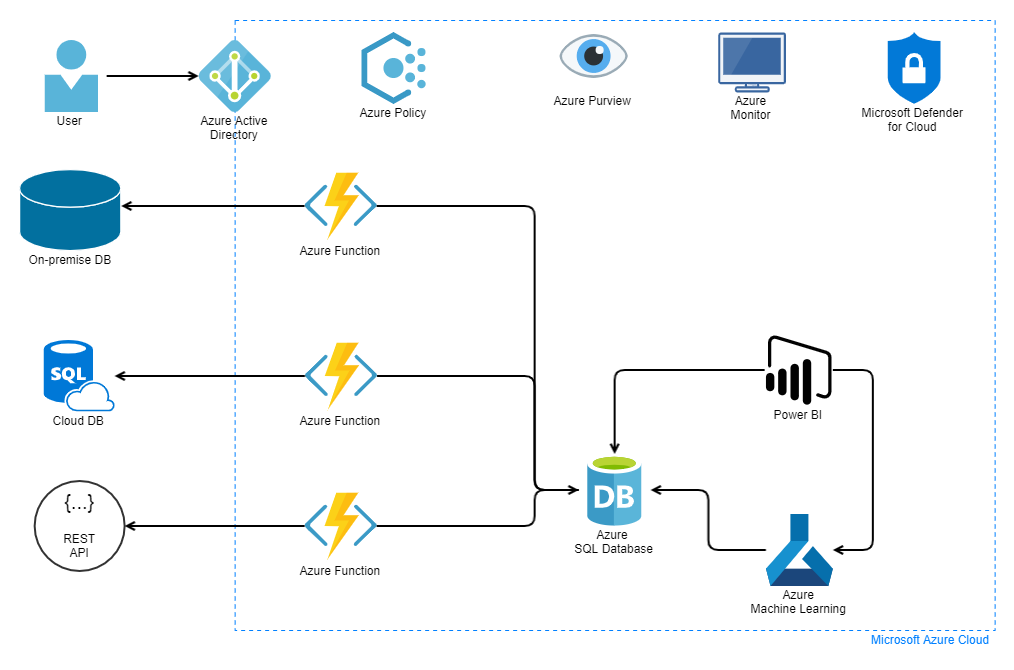
\includegraphics[width=\textwidth]{gfx/chap03_konzept_architektur.png}
 \caption{Konzept für BI-Architektur in Azure Cloud (Entwurf)}
\label{fig:chap03_4_konzeptArchitektur}
\end{figure}

\textit{...}